\documentclass[11pt]{article}
\usepackage[a4paper,margin=28mm]{geometry}
\usepackage{amsmath,amssymb,amsthm,mathtools,microtype,mathrsfs}
\usepackage{tikz}
\usetikzlibrary{arrows.meta,positioning,calc}
\usepackage[colorlinks=true,linkcolor=blue!55!black,urlcolor=blue!55!black,citecolor=blue!55!black]{hyperref}
\newtheorem{theorem}{Theorem}[section]
\newtheorem{proposition}[theorem]{Proposition}
\newtheorem{lemma}[theorem]{Lemma}
\newtheorem{definition}[theorem]{Definition}
\newtheorem{corollary}[theorem]{Corollary}
\theoremstyle{remark}\newtheorem{remark}[theorem]{Remark}
\numberwithin{equation}{section}
\newcommand{\ii}{\mathrm i}
\newcommand{\dd}{\,\mathrm d}
\newcommand{\Turn}{\mathcal T}
\newcommand{\core}{\mathrm{core}}
\newcommand{\arccot}{\operatorname{arccot}}
\newcommand{\Ti}{\operatorname{Ti}_2}
\newcommand{\supp}{\operatorname{supp}}
\title{Complementary color bounds for Conway tangle sources}
\author{}
\date{}
\begin{document}
\maketitle
\begin{abstract}
An auxiliary circle in a root-of-unity tangle evaluation has a finite Newton expansion with a low-index core and an exact complementary term. A retained half twist mixes its coefficients and introduces cancellation. We prove that every contribution containing a complementary term is exponentially smaller than the positive complete-color source for a fixed Conway construction whose closing boxes are both completed. The estimate is uniform over all physical auxiliary colors, both parities of the level, and every fixed choice of retained half-twist signs. A second estimate controls the entire source when one color stays a fixed fraction of the level away from complete color. The proof derives a finite recurrence for the actual coefficients, bounds both recurrence roots through their collisions, and propagates two strict local comparisons through the original construction. The local comparisons are certified by outward rational arithmetic on complete slope polytopes. No asymptotic assertion about a filled invariant is needed.
\end{abstract}

\section{The source and the result}\label{cs:intro}

A circle surrounding two strands can be evaluated before it is filled by twists. The resulting two-strand operator depends on the dimension assigned to that circle. At complete color its turned Newton coefficients are positive. Other colors contain an additional signed polynomial, which remains present in the exact finite source. Bounding only the complete-color coefficients therefore leaves a necessary part of the evaluation uncontrolled.

We work with a fixed construction from elementary circle tangles, vertical stacking and clockwise quarter turns. The construction is \emph{completed} if it is obtained by the following rules: a stack of two elementary pieces is completed; the turn of a completed box is completed; a stack of two completed boxes is completed; and attaching one elementary piece above or below a completed box is completed. A closed construction consists of two completed boxes joined by cylindrical closure. These are the diagrams of \cite[Definition 2.1]{Newton}. The construction, the number of its elementary pieces, and their retained crossing signs are fixed as the level grows. The two completed closing boxes are an essential hypothesis.

Here an elementary piece is a colored auxiliary circle in its disk framing, followed by the prescribed turn. It may retain no crossing, one positive crossing or one negative crossing in that disk. Write its sign as $\epsilon\in\{0,1,-1\}$. The term \emph{physical color} means an integer dimension $j$ with $1\le j\le N$. It does not mean a freely chosen continuous parameter.

At each elementary piece the exact polynomial is the sum of a core and a complementary polynomial, which we call its \emph{alias}. Section~\ref{cs:finite} defines this split, including low colors for which the core is zero. Let $\mathcal A_N(\mathbf j,\boldsymbol\epsilon)$ be the scalar obtained by the original turns, stacks and closing trace. Let $\mathcal C_N(\mathbf j,\boldsymbol\epsilon)$ be the same expression with every elementary piece replaced by its core. Both are finite, exact expressions in the full root algebra. Define $F_0$ to be the maximum action of the pure complete-color construction: every $j=N$ and every $\epsilon=0$.

\begin{theorem}[Uniform complementary and color gaps]\label{cs:main}
Fix a completed closed construction. There are $\gamma>0$ and $N_0$ such that, for all $N\ge N_0$ and all its physical colors and retained signs,
\begin{equation}\label{cs:alias-gap}
 |\mathcal A_N(\mathbf j,\boldsymbol\epsilon)-\mathcal C_N(\mathbf j,\boldsymbol\epsilon)|
 \le \exp\{N(F_0-\gamma)\}.
\end{equation}
For every $\delta>0$ there are $\gamma_\delta>0$ and $N_\delta$ such that
\begin{equation}\label{cs:color-gap}
 \max_\ell(N-j_\ell)\ge\delta N
 \quad\Longrightarrow\quad
 |\mathcal A_N(\mathbf j,\boldsymbol\epsilon)|
 \le\exp\{N(F_0-\gamma_\delta)\},\qquad N\ge N_\delta.
\end{equation}
The limits range over all integer levels, including composite levels. Constants may depend on the fixed construction and on $\delta$; no uniformity over growing trees is asserted.
\end{theorem}

The proof has three different comparisons. First, the exact finite algebra identifies which coefficients occur. Second, a positive majorant controls all core coefficients, even at colors where a recurrence has repeated characteristic roots. Third, strict inequalities for a two-leaf block and a single attachment leave a loss that survives the whole construction. The final estimate concerns a sum of all alias selections, rather than one favorable contribution.

Theorem~\ref{cs:main} is an upper bound for the source before filling. A nonzero asymptotic for a selected filled contribution and an exact filling transformation are additional inputs to any filled-invariant conclusion. In particular the theorem alone neither identifies a hyperbolic volume nor rules out cancellation inside the retained core.

\subsection{Precise imported results}
We use the following numbered results of \emph{Newton coefficients and positive sources for Conway tangles} \cite{Newton}. Proposition 3.2 identifies the physical turn and trace in the normalized Newton basis; Theorem 3.3 gives multiplication in the full quotient, including repeated-root derivatives. Proposition 4.1 and equations (4.4)--(4.8) give the colored-circle split and the two retained crossing operators. We display these formulas below so that all subsequent estimates have explicit inputs. Proposition 5.3 gives the unique strict maximum of the positive complete source; Lemma 6.1 locates every selected leaf in
\begin{equation}\label{cs:leaf-window}
 \frac14<a<\frac{\arctan 2}{\pi}<\frac12
\end{equation}
and gives the boundary-parameter inequalities used in Section~\ref{cs:attachment}. The positive variational theorem uses the actual finite lattice, with no restriction to a subsequence of levels. No complex interpolation theorem is imported here.

\section{Exact finite coefficients and their supports}\label{cs:finite}

Put $d=N-1$, $M=\lfloor d/2\rfloor$, $q=e^{\pi\ii/N}$ and $Q=q^2$. Throughout this paper
\[
 S_r=\prod_{a=1}^r2\sin(\pi a/N),\qquad S_0=1,
 \qquad c_a=q^{2a+1}+q^{-2a-1}.
\]
Thus $S_r$ is a product, not a single sine. The root algebra is
\[
 \mathscr A_N=\mathbb C[z]/(P_N(z)),\qquad
 P_N(z)=2T_N(z/2)+2=\prod_{a=0}^{d}(z-c_a),
\]
where $T_N(\cos t)=\cos Nt$. Repeated entries in the displayed product remain repeated roots. Equality in $\mathscr A_N$ preserves values and first derivatives at its double roots; at odd $N$ the simple root $-2$ also remains.
The normalized Newton basis is
\begin{equation}\label{cs:basis}
 e_r(z)=S_r^{-2}\prod_{a=0}^{r-1}(c_a-z),\qquad 0\le r\le d.
\end{equation}
The physical clockwise turn $\Turn$ and normalized cylindrical closure $\phi$ satisfy
\begin{equation}\label{cs:turn-trace}
 \Turn e_r=e_{d-r},\qquad \phi(e_i e_j)=\mathbf1_{i+j=d}.
\end{equation}
A stack is multiplication. For $i+j\le d$ its exact coefficients are
\begin{equation}\label{cs:product}
 e_i e_j=\sum_{k=\max(i,j)}^{i+j}
 \frac{S_{i+j}S_k}{S_iS_jS_{k-i}S_{k-j}S_{i+j-k}}e_k.
\end{equation}
For $i+j\ge N$ the product is zero in the full algebra, with multiplicities. All nonzero coefficients in \eqref{cs:product} are positive. We call one use of this multiplication a \emph{gate}. Its exact finite support is
\begin{equation}\label{cs:support}
 i,j\ge0,\qquad i+j\le d,\qquad \max(i,j)\le k\le i+j.
\end{equation}
At a closing gate the trace forces $i+j=d$, and its coefficient is one. This is an exact constraint before any scaling by $N$.

\subsection{The core and the alias}
Let $U_0(z/2)=1$, $U_1(z/2)=z$, and $U_{r+1}(z/2)=zU_r(z/2)-U_{r-1}(z/2)$. The ordinary circle is $L_j=(-1)^{j-1}U_{j-1}(z/2)$, and the elementary turned piece is $h_j=\Turn L_j$. Put $h_0=0$. For a high color $j=N-h$, $0\le h\le M$, its exact split is
\begin{align}
 h_{N-h}&=C_{N-h}+A_{N-h},\\
 C_{N-h}&=\sum_{v=h}^{M}
 \frac{N^2S_{2v}}{S_v^2S_{v-h}S_{v+h}}e_v,
 &A_{N-h}&=(-1)^N h_h.\label{cs:split}
\end{align}
For the remaining physical colors $1\le j\le\lfloor N/2\rfloor$, set $C_j=0$ and $A_j=h_j$. The low-color formula is
\begin{equation}\label{cs:low-color}
 h_j=\sum_{r=0}^{j-1}(-1)^{j-1+r}
 \frac{S_r^2S_{j+r}}{S_{2r+1}S_{j-r-1}}e_{d-r}.
\end{equation}
There is no overlap or omitted color in this definition. The high and low \emph{colors} should be distinguished from the high and low \emph{Newton indices}: the high-color core has indices at most $M$, while an alias before the retained half twist in \eqref{cs:low-color} has indices $d-r\ge N/2$.

Let $\kappa=q^{d^2/2}$, with $q^a=e^{\pi\ii a/N}$ for real $a$. A retained half twist acts by
\begin{equation}\label{cs:half-twist}
 \Theta_\epsilon e_v=\kappa^\epsilon(-1)^v
 \sum_{r=0}^v q^{\epsilon v(r+1)}
 \frac{S_v}{S_rS_{v-r}}e_r,\qquad \epsilon=\pm1,
 \qquad \Theta_0=1.
\end{equation}
Define $C_j^\epsilon=\Theta_\epsilon C_j$ and $A_j^\epsilon=\Theta_\epsilon A_j$. The core still has indices at most $M$, but a half-twisted alias can occupy every index from $0$ to $d$. Thus the alias must be estimated on the entire gate support \eqref{cs:support}. The phases in \eqref{cs:half-twist} are retained until after the finite sum has been formed.

Equations \eqref{cs:turn-trace}--\eqref{cs:half-twist} are the physical identities imported above. Their derivation in \cite{Newton} is in the full quotient, not merely at the distinct roots. Consequently the estimates below concern the original normal data too; no semisimple replacement of a circle is made.

\subsection{Continuous actions and elementary bounds}\label{cs:actions}
Define the continuous function
\[
 J(t)=\int_0^t\log(2\sin\pi u)\dd u,\qquad 0\le t\le1.
\]
It satisfies $J(1-t)=-J(t)$ and $J(0)=J(1/2)=J(1)=0$. The leaf and gate actions are
\begin{align}
 g(x)&=J(2x)-4J(x),&0\le x\le\tfrac12,\label{cs:g}\\
 m(x,y,z)&=J(x+y)+J(z)-J(x)-J(y)\notag\\[-2mm]
 &\quad-J(z-x)-J(z-y)-J(x+y-z).\label{cs:m}
\end{align}
The full limiting gate polytope is
\begin{equation}\label{cs:D}
 D=\{x,y\ge0:\ \max(x,y)\le z\le x+y\le1\}.
\end{equation}
It includes inputs larger than $1/2$. The two majorant profiles will be
\begin{equation}\label{cs:profiles}
 \widetilde g(x)=g(\max(x,1/4))\quad(0\le x\le1/2),
 \qquad k(x)=-2J(x/2)\quad(0\le x\le1).
\end{equation}

For reference, the uniform sine-factorial estimate is
\begin{equation}\label{cs:factorial}
 \log S_r=NJ(r/N)+O(\log N),\qquad 0\le r<N.
\end{equation}
To see endpoint uniformity, subtract $\log t+\log(1-t)$ from the integrand of $J$. The remainder extends with a bounded derivative to $[0,1]$, so its Riemann sum has bounded error. The two removed sums are logarithms of ordinary factorials; integral comparison, or Stirling's inequalities, bounds their errors by $O(\log N)$ uniformly in the endpoint. This includes $r=0$. Applied to \eqref{cs:product}, it gives the exponent $Nm(i/N,j/N,k/N)$ with a uniform $O(\log N)$ error.

All three profiles $\widetilde g,k,m$ are concave on their indicated domains. Indeed
\[
\begin{aligned}
 g'(x)&=2\log\cot\pi x,&g''(x)&<0,\\
 k'(x)&=-\log(2\sin(\pi x/2)),&
 k''(x)&=-\frac\pi2\cot(\pi x/2)<0.
\end{aligned}
\]
The derivative of $\widetilde g$ is zero on its plateau and joins $g'$ continuously at $1/4$. For the gate put $p=z-x$, $q_1=z-y$, $r=x+y-z$, $w=1-x-y$. Then
\begin{equation}\label{cs:tetrahedra}
 \pi m=V(y,x,w)+V(p,q_1,2r+w)+V(p+q_1,r,r+w),
 \qquad V(a,b,c)=-\pi[J(a)+J(b)+J(c)].
\end{equation}
Each triple is nonnegative and sums to one. On such a triangle $V$ is concave: its two-variable negative Hessian is a positive multiple of
$\left(\begin{smallmatrix}\cot\pi a+\cot\pi c&\cot\pi c\\\cot\pi c&\cot\pi b+\cot\pi c\end{smallmatrix}\right)$, whose diagonal entries are positive and whose determinant is one. Continuity handles the boundary. Identity \eqref{cs:tetrahedra}, obtained by $J(1-t)=-J(t)$, proves concavity on the full $D$.

\section{Uniform bounds for one actual leaf}\label{cs:local}

The difficult coefficient is a half-twisted core. Taking the absolute value of each term in \eqref{cs:half-twist} would lose the cancellation needed for its correct exponential rate. We derive a recurrence for that signed finite sum, including its endpoint condition, and then bound products of its recurrence matrices.

\begin{proposition}[Leaf envelopes]\label{cs:envelopes}
There are a sequence $e_N\to0$ and an absolute constant $C$ such that, uniformly over all physical colors and $\epsilon\in\{0,1,-1\}$,
\begin{align}
 |[e_r]C_j^\epsilon|&\le
 \exp\{N[\widetilde g(r/N)+e_N]\},&&0\le r\le M,\label{cs:core-envelope}\\
 |[e_r]A_j^\epsilon|&\le N^C\exp\{Nk(r/N)\},&&0\le r\le d.\label{cs:alias-envelope}
\end{align}
The core is zero above $M$. Moreover, if $I\subset(1/4,1/2)$ is compact and $\delta>0$, there is $\eta>0$ such that, for all sufficiently large $N$,
\begin{equation}\label{cs:local-color-loss}
 h\ge\delta N,\quad r/N\in I,\quad 0\le h\le M
 \quad\Longrightarrow\quad
 |[e_r]C_{N-h}^\epsilon|
 \le\exp\{N[g(r/N)-\eta]\}.
\end{equation}
Zero coefficients are included. No polynomial prefactor for the core is asserted at collisions of recurrence roots.
\end{proposition}

\subsection{The finite Ward identity}
Here $F_r=(Q;Q)_r=\prod_{a=1}^r(1-Q^a)$, $F_0=1$. For integers $0\le h,r\le M$ put
\begin{align}
 A_{h,r}&=\sum_{v=\max(r,h)}^M
 \frac{Q^{-vr}F_{2v}}{F_vF_{v-h}F_{v+h}F_{v-r}},\label{cs:finite-A}\\
 D_{0,r}&=\frac{Q^{-r^2}F_{2r}}{F_r^3},
 &V_{h,r}&=\frac{q^{h^2}A_{h,r}}{D_{0,r}}.\label{cs:finite-V}
\end{align}
Every factorial in these sums has a nonnegative index below $N$, and $D_{0,r}\ne0$. The lower endpoint is $\max(r,h)$ even when the output index is below the color deficit.

The elementary phase identity
\[
 F_a=(-\ii)^a q^{a(a+1)/2}S_a
\]
converts the negative half-twist coefficient in \eqref{cs:half-twist} to
\[
 [e_r]C_{N-h}^{-1}
 =\frac{N^2\kappa^{-1}}{S_r}\,
 \ii^r q^{(r^2-r)/2+h^2}A_{h,r}.
\]
The positive sign is its complex conjugate in the real Newton basis. Thus
\begin{equation}\label{cs:exact-modulus}
 |[e_r]C_{N-h}^{\epsilon}|=
 \frac{N^2S_{2r}}{S_r^4}|V_{h,r}|,
 \qquad \epsilon=\pm1.
\end{equation}
This is the modulus of the original sum, after its phases have been combined.

Set $H=Q^h$, $Y=Q^r$ and $T_h=H+H^{-1}$. The exact finite sum satisfies
\begin{multline}\label{cs:Ward}
 QY^2(1-Q^2Y)A_{h,r+2}
 +Y(T_hQ^3Y^2+Q+1)A_{h,r+1}\\
 -Q(QY+1)(QY^2-1)A_{h,r}=0.
\end{multline}
Absent sums above $M$ are zero. Here is an explicit telescoping proof. If $z=Q^v$, the ratio of consecutive summands of \eqref{cs:finite-A} is
\[
 R(z)=\frac{Y^{-1}(1-Qz^2)(1+Qz)}
 {(1-Qz/H)(1-QHz)(1-Qz/Y)}.
\]
Use
\[
 G_h(z)=\frac{(1-z/H)(1-Hz)(1-z/Y)}{z^2}.
\]
Expanding $R(z)G_h(Qz)-G_h(z)$ gives
\begin{equation}\label{cs:telescoper}
 \left(\frac1{YQ^2}-1\right)z^{-2}
 +\left(\frac1{YQ}+H+H^{-1}+\frac1Y\right)z^{-1}
 -\frac1{YQ}-1-\frac{H+H^{-1}}Y.
\end{equation}
The ratio of a summand at $r+1$ to its value at $r$ is $z^{-1}-Y^{-1}$. Applying this identity twice expresses the first two $z^{-1}$ moments in terms of $A_{h,r+1}$ and $A_{h,r+2}$ and gives \eqref{cs:Ward} after clearing the displayed denominators.

The endpoints vanish in this cleared form. At $v=\max(r,h)$ one of $1-z/Y$ and $1-z/H$ is zero. At the upper endpoint, multiplying the next summand by $G_h(Q^{M+1})$ first cancels the three last factorial factors; the remaining numerator contains $F_{2M+2}$ and hence $1-Q^N$. This order also covers $h=M$, where an uncanceled ratio would read $0/0$. No negative factorial or division by a zero endpoint is used. These observations prove the recurrence for $r<h$ as well as $r\ge h$.

Normalizing by \eqref{cs:finite-V} and writing $Z=Q^{r+1}$ gives
\begin{align}
 V_{h,r}&=p_{h,N}(r)V_{h,r+1}+q_N(r)V_{h,r+2},\label{cs:recurrence}\\
 p_{h,N}(r)&=-\frac{Z^{-1}[(H+H^{-1})Z^2+1+Q^{-1}]}{(1-Z)^2},\notag\\
 q_N(r)&=-\frac{Q^{-2}Z^{-2}(1-QZ^2)(1+QZ)}
 {(1-Z)^2(1-QZ)}.\notag
\end{align}
The denominators are nonzero for $0\le r\le M-1$. At $r=M-1$, $q_N(r)=0$ at both parities. We may set the unused value $V_{h,M+1}=0$. The actual remaining terminal value is
\begin{equation}\label{cs:terminal}
 |V_{h,M}|=\frac{S_M^2}{S_{M-h}S_{M+h}}
 =\begin{cases}1,&N\text{ odd},\\ \cos(\pi h/N),&N\text{ even}.
 \end{cases}
\end{equation}
Indeed $S_aS_{N-1-a}=N$. For odd $N=2M+1$ both products in the ratio equal $N$. For even $N=2m$, $M=m-1$, the numerator is $N/2$ and the denominator is $N/(2\cos(\pi h/N))$. Thus the prescribed solution is bounded by one at the upper wall throughout the physical color range. For the rate arguments it suffices to take $N\ge3$; the finite formulas still have their stated meaning at $N=2$.

\subsection{Both roots of the recurrence}
Let $T_N(r)$ be the companion matrix of \eqref{cs:recurrence}, so that
$(V_{h,r},V_{h,r+1})^{\mathsf t}=T_N(r)(V_{h,r+1},V_{h,r+2})^{\mathsf t}$.
Freeze $u=(r+1)\pi/N$ and $\chi=\pi h/N$ while $Q\to1$. The limiting matrix $T_0(u,\chi)$ has eigenvalues $e^{-2\ii u}v$, where
\begin{equation}\label{cs:ellipse-polynomial}
 v^2-bv-c=0,\qquad c=\cot^2u,\qquad
 b=(c-1)\cos^2\chi-2\ii\sqrt c\sin^2\chi.
\end{equation}
We claim
\begin{equation}\label{cs:spectral-radius}
 \rho(T_0(u,\chi))\le\rho_0(u):=\max(1,\cot^2u),
 \qquad 0<u\le\pi/2,\quad0\le\chi\le\pi/2.
\end{equation}
For $0<c<1$, a root $v$ on the unit circle would require $b=v-c/v$. Its locus in the $b$ plane is the ellipse
\[
 \left(\frac{\Re b}{1-c}\right)^2+
 \left(\frac{\Im b}{1+c}\right)^2=1.
\]
At the actual $b$ its left side is
\[
 \cos^4\chi+\frac{4c}{(1+c)^2}\sin^4\chi\le1,
\]
with strict inequality for $\chi>0$. At the center the roots have modulus $\sqrt c<1$. Along a segment inside the ellipse no root can cross the unit circle, proving the bound for both roots. Continuity covers its boundary. For $c>1$ apply the same argument to $v/c$ and $1/c$. At $c=1$ the roots of $v^2+2\ii\sin^2\chi\,v-1$ have modulus one; at $c=0$ they are $0$ and $-\cos^2\chi$. This proves \eqref{cs:spectral-radius}.

In particular, for $\chi_0>0$ and a compact interval $I\subset(\pi/4,\pi/2)$,
\begin{equation}\label{cs:strict-radius}
 \sup_{u\in I,\,\chi_0\le\chi\le\pi/2}\rho(T_0(u,\chi))
 \le\theta<1.
\end{equation}
The endpoint $\chi=\pi/2$ is included: its repeated root has modulus $\sqrt c<1$. We will bound matrix powers directly, without an eigenbasis that could become singular there.

\subsection{Fixed blocks and the lower endpoint}
Define
\begin{equation}\label{cs:E}
 E(u)=\begin{cases}\displaystyle\frac2\pi\int_u^{\pi/4}\log\cot t\dd t,
 &0\le u<\pi/4,\\0,&\pi/4\le u\le\pi/2.
 \end{cases}
\end{equation}
The recurrence implies
\begin{align}
 \limsup_{N\to\infty}\max_{0\le h,r\le M}
 \{N^{-1}\log|V_{h,r}|-E(\pi r/N)\}&\le0,\label{cs:global-V}\\
 \limsup_{N\to\infty}
 \max_{\substack{\delta N\le h\le M\\0\le r\le\beta N}}
 \{N^{-1}\log|V_{h,r}|-E(\pi r/N)\}&\le-\gamma_{\delta,\beta}<0,
 \label{cs:strict-V}
\end{align}
for $0<\delta,\beta<1/2$. We use $\log0=-\infty$ and ignore an empty index set.

Here are the uniform product estimates. Fix a lower cutoff $a>0$. For $a\le u_r=(r+1)\pi/N\le\pi/2$, the exact normalized matrices
$B_N(r)=T_N(r)/\rho_0(u_r)$ differ by $O_a(N^{-1})$ from the bounded Lipschitz family $B(u_r,\chi)=T_0(u_r,\chi)/\rho_0(u_r)$. The factor $1-QZ$ in \eqref{cs:recurrence} stays bounded away from zero on this interval at all sufficiently large levels.

For a bounded $2$ by $2$ matrix whose eigenvalues have modulus at most one, Cayley--Hamilton gives
\begin{equation}\label{cs:matrix-power}
 \|B^L\|\le L\|B\|+L-1\le C_a L.
\end{equation}
The coefficient of $B$ is the polynomial
$\sum_{j=0}^{L-1}\lambda_1^{L-1-j}\lambda_2^j$; the constant coefficient has modulus at most $L-1$. The formula extends to equal roots. If both roots have modulus at most $\theta<1$, it gives $\|B^L\|\le C_a L\theta^{L-1}$.

Choose a fixed integer $L$. Telescoping the product of $L$ adjacent matrices against its frozen value gives, uniformly in $\chi$,
\[
 B_N(r)\cdots B_N(r+L-1)
 =B(u_r,\chi)^L+O_{a,L}(N^{-1}).
\]
For a prescribed $\varepsilon>0$, choose $L$ large enough that $C_aL<e^{\varepsilon L}$ and only then take $N$ sufficiently large. Complete blocks cost at most $e^{2\varepsilon L}$; the incomplete blocks at the ends cost a fixed constant. Thus any normalized propagation above the cutoff costs at most $C_{a,\varepsilon}e^{2\varepsilon N}$.

For \eqref{cs:strict-V}, choose
$I\subset(\max(\pi\beta,\pi/4),\pi/2)$. Propagation from the upper wall to any $r\le\beta N$ crosses $I$. Equation \eqref{cs:strict-radius} permits the same fixed $L$ to be enlarged until every full block inside $I$ has norm at most $e^{-\gamma_0 L}$ for some $\gamma_0>0$. There are $N|I|/(\pi L)+O(1)$ such blocks. Taking $\varepsilon<\gamma_0|I|/(8\pi)$ leaves a strict negative rate after the remaining blocks have been included.

At the omitted lower endpoint, direct estimates in \eqref{cs:recurrence} give
\[
 \|T_N(r)\|\le C\frac{N^2}{(r+1)^2},\qquad u_r\le a<\pi/8.
\]
Indeed $|H+H^{-1}|\le2$, $|1-Z|\ge4(r+1)/N$, and
$|1-QZ^2|/|1-QZ|$ is bounded in this range. For at most $K\le aN/\pi$ consecutive indices the product is bounded by
\[
 \frac{C^KN^{2K}}{(K!)^2}
 \le\exp\{O(Na\log(1/a))+O(\log N)\}.
\]
This also covers a shorter segment beginning later, by enlarging the absolute constant so each omitted factor is at least one. Its normalized rate tends to zero with $a$.

Finally $\log\rho_0$ decreases to zero, so its right-endpoint Riemann sum satisfies
\[
 \sum_{j=r}^{M-1}\log\rho_0((j+1)\pi/N)\le NE(\pi r/N).
\]
For the global assertion first fix $a$ and $\varepsilon$, then $L$, then $N$, and finally make $a,\varepsilon$ arbitrarily small. For the strict assertion fix $I$ and its negative budget first; choose $a\log(1/a)$ and $\varepsilon$ below that budget, then $L$, and finally $N$. Combining \eqref{cs:terminal} with these estimates proves \eqref{cs:global-V} and \eqref{cs:strict-V}. Both branches, including their collisions, have been bounded.

The prefactor in \eqref{cs:exact-modulus} has rate $g(x)$ by \eqref{cs:factorial}, and
\begin{equation}\label{cs:plateau}
 g(x)+E(\pi x)=g(\max(x,1/4))=\widetilde g(x).
\end{equation}
This proves \eqref{cs:core-envelope} for the two twisted signs. For an untwisted core, the coefficient vanishes for $r<h$ and otherwise has rate
\[
 g(x)-\Delta(x,t),\qquad
 \Delta(x,t)=J(x-t)+J(x+t)-2J(x),
 \quad t=h/N,\ x=r/N.
\]
For $t>0$ and $x<1/2$,
\[
 \partial_t\Delta=\log\frac{\sin\pi(x+t)}{\sin\pi(x-t)}>0,
\]
since the difference of the two sines is $2\cos\pi x\sin\pi t>0$. The boundary $t=x$ is integrable and follows by continuity. This proves the untwisted bound and its strict loss on a fixed high interval when $t\ge\delta$. For the twisted signs, choose $\beta$ above that interval and apply \eqref{cs:strict-V}; $E=0$ there. Thus \eqref{cs:local-color-loss} follows at both parities.

\subsection{The full alias range}
It remains to prove \eqref{cs:alias-envelope}. The absolute value of a coefficient in \eqref{cs:low-color} is
\[
 b_{j,r}=\frac{S_r^2}{S_{2r+1}}
 \prod_{a=-r}^r2\sin((j+a)\pi/N),\qquad
 0\le r<j\le\lfloor N/2\rfloor.
\]
As a function of real $j$ on $(r,N-r)$, the logarithm of the product is strictly concave and symmetric about $N/2$. Its maximum is at that center. Sine duplication gives
\[
 b_{j,r}\le B_r:=
 2\frac{\prod_{a=1}^r2\sin(2a\pi/N)}
 {\prod_{a=0}^r2\sin((2a+1)\pi/N)}.
\]
Here $B_0=\csc(\pi/N)$ and
$B_{r+1}/B_r=\sin((2r+2)\pi/N)/\sin((2r+3)\pi/N)$.
The ratio changes from at most one to at least one at most once, so a maximum occurs at an endpoint. The last value is $N/2$ for even $N$, and $\csc(\pi/N)$ for odd $N$. Since $\sin(\pi/N)\ge2/N$,
\begin{equation}\label{cs:raw-alias}
 b_{j,r}\le N/2.
\end{equation}

A half twist contributes a coefficient ratio $S_v/(S_rS_{v-r})$, where $v\ge\max(r,N/2)$. Its rate is
\[
 J(w)-J(u)-J(w-u),\qquad w=v/N,\ u=r/N.
\]
Differentiation in $w$ gives
$\log(\sin\pi w/\sin\pi(w-u))$; its maximum is at $w=(1+u)/2$. Reflection and duplication of $J$ give the maximum $-2J(u/2)=k(u)$. Uniform factorial errors and at most $N$ summands cost only a power of $N$. This proves \eqref{cs:alias-envelope} for both twists. The pure alias obeys the same bound because $k\ge0$ and \eqref{cs:raw-alias} applies. Proposition~\ref{cs:envelopes} is proved.

\section{A two-leaf comparison on the whole output interval}\label{cs:two-leaf}

In a completed pure reference the selected leaf range is
\begin{equation}\label{cs:leaf-window}
 \frac14<a<\frac{\arctan2}{\pi}<\frac12.
\end{equation}
A pointwise comparison with a single complete leaf is insufficient
throughout this range. The relevant quantity would be
\[
 \min_{0\le u\le1}\{g(a)+g'(a)(u-a)-k(u)\},
\]
which need not be positive there. The gate joining two leaves supplies the missing comparison. We retain it, and its output tangent, before propagating an estimate into the rest of the tree.

At the selected pure two-leaf stack, write
\begin{equation}\label{cs:seed-parameters}
 X=\cot\pi a,\qquad \cot\pi b=X-\frac1{2X},\qquad
 F_2(b)=2g(a)+m(a,a,b),\qquad
 \lambda=2\log(2X^2).
\end{equation}
Here $\arccot$ takes values in $(0,\pi)$. The displayed expressions define the scalar parameters for every $X\in[1/2,1]$. Completed pure references use the interior range; the three-leaf reference in Section~\ref{cs:probe} uses the endpoint $X=1/2$.

\begin{lemma}[Two-leaf gap]\label{cs:two-leaf-gap}
For $1/2\le X\le1$ and the slope in \eqref{cs:seed-parameters},
\begin{align}
 \max_{D,\,y\le1/2}
 \{k(x)+\widetilde g(y)+m(x,y,z)-\lambda z\}
 &\le F_2(b)-\lambda b-\frac1{100},\label{cs:AC}\\
 \max_D\{k(x)+k(y)+m(x,y,z)-\lambda z\}
 &\le F_2(b)-\lambda b-\frac1{100}.\label{cs:AA}
\end{align}
\end{lemma}

\begin{proof}
Let $P(\lambda)$ be the maximum of $g(x)+g(y)+m(x,y,z)-\lambda z$ on $D$ with $x,y\le1/2$. Direct differentiation at $(a,a,b)$ gives
\[
 m_x=m_y=-2\log X,\qquad m_z=\lambda,\qquad g'(a)=2\log X.
\]
This point is strict in $D$, including the endpoints $X=1/2,1$. Concavity proves
\[
 P(\lambda)=F_2(b)-\lambda b.
\]
The same maximum is obtained if either or both copies of $g$ are replaced by $\widetilde g$: the selected point has $a\ge1/4$, where their supporting tangents agree.

We give the complete finite certificate reduction. Write $H=k+\widetilde g+m$ for the first alias action and $H=k+k+m$ for the second. A rational feasible pure point $p=(p_1,p_1,p_3)$ gives
\[
 P(\lambda)\ge 2g(p_1)+m(p)-\lambda p_3.
\]
For a strict rational alias point $v$, with $v_2>1/4$ in the first case, global concavity gives
$H(w)\le H(v)+\nabla H(v)\cdot(w-v)$. The full vertex sets are
\begin{align*}
 \mathcal V_{\mathrm{AC}}={}&
 \{(0,0,0),(1,0,1),(1/2,1/2,1/2),(0,1/2,1/2),(1/2,1/2,1)\},\\
 \mathcal V_{\mathrm{AA}}={}&
 \{(0,0,0),(1,0,1),(0,1,1),(1/2,1/2,1/2)\}.
\end{align*}
To verify that these lists are complete, the nonnegative coordinates
$p=z-x$, $q_1=z-y$, $r=x+y-z$, $w_0=1-x-y$ obey
$p+q_1+2r+w_0=1$. Thus $D$ is a tetrahedron. Cutting by $y\le1/2$ removes one vertex and adds the two listed edge intersections.

Partition $\lambda/\log2\in[-2,2]$ into the sixteen intervals
$[-2+j/4,-2+(j+1)/4]$, $j=0,\ldots,15$. On each interval the rational data in \cite{Certificates} give one pure point and one tangent point for each alias action. For every vertex $w$ and the two slope endpoints $t$, they give
\begin{equation}\label{cs:two-certificate}
 2g(p_1)+m(p)-t\log2\,p_3
 -H(v)-\nabla H(v)\cdot(w-v)+t\log2\,w_3>\frac1{100}.
\end{equation}
The expression is affine separately in the slope and in $w$. Its endpoint and vertex checks therefore prove the inequality on each full interval and polytope. There are $16\cdot2\cdot(5+4)=288$ inequalities. Section~\ref{cs:arithmetic} proves the outward enclosure rules and specifies the exact data. The smallest certified lower bound is
\begin{equation}\label{cs:two-margin}
 \frac{210002102902309638093785766005979344329}
 {5000000000000000000000000000000000000000}
 >\frac1{25}>\frac1{100}.
\end{equation}
This proves both comparisons, including boundary maxima and the core plateau.
\end{proof}

\section{A new leaf and an arbitrary completed child}\label{cs:attachment}

A completed child is represented by its actual selected output and its output derivative. Its entire internal source remains in the calculation. Let $f_E(b)$ be its optimized pure complete action at output $b$, near the selected strict state. The imported strict maximum has negative Hessian in its internal variables, so the implicit function theorem gives this differentiable local profile. Its derivative is the boundary Lagrange multiplier.

The boundary variables from \cite[Section 6]{Newton} are
\[
 B=\cot\pi b,\qquad
 X^2=\frac{1+B^2}{1+e^{-f_E'(b)}},\qquad
 Y=e^{-f_E'(b)/2}X.
\]
Thus $X^2+Y^2-B^2=1$ and $f_E'(b)=2\log(X/Y)$. At a stack the two children have the same $X$, and their output variables satisfy
\[
 B_o=\frac{B_1B_2+X^2-1}{B_1+B_2},
 \qquad Y_o=\frac{Y_1Y_2}{B_1+B_2}.
\]
For a leaf attached to a completed child these become
\begin{equation}\label{cs:attachment-parameters}
 \begin{gathered}
 a=\arccot X/\pi,\quad b=\arccot B/\pi,\quad
 c=\arccot B_p/\pi,\quad B_p=X-\frac1{X+B},\\
 Y_p=\frac{Y}{X+B},\qquad
 \mu=f_E'(b)=2\log(X/Y),\qquad
 \lambda=f_{hE}'(c)=2\log(X/Y_p).
 \end{gathered}
\end{equation}
For a completed pure reference, both child and parent are completed. Lemma 6.1 of \cite{Newton} then gives $0<X,Y,Y_p<1$. The child inequality $Y<1$ gives $|B|<X$. The parent inequality $Y_p<1$ gives
\[
 B>\frac1{2X}-X.
\]
Together they force $X>1/2$. These two distinct inequalities are needed below.

Define the pure and alias dual maxima
\begin{align}
 P(\mu,\lambda)&=\max_{D,\,x\le1/2}
 \{g(x)+m(x,y,z)+\mu y-\lambda z\},\label{cs:single-P}\\
 Q(\mu,\lambda)&=\max_D
 \{k(x)+m(x,y,z)+\mu y-\lambda z\}.\label{cs:single-Q}
\end{align}
Only the new leaf has the restriction $x\le1/2$. The child coordinate $y$ retains the whole interval $[0,1]$; it is represented by its tangent, not replaced by a second leaf.

\begin{lemma}[Single-attachment gap]\label{cs:attachment-gap}
Let $1/2<X<1$, $Y=\sqrt{1+B^2-X^2}$, $Y_p=Y/(X+B)$ and $0<Y,Y_p<1$, with the positive branch $X+B>0$. Define $a,b,c,\mu,\lambda$ by \eqref{cs:attachment-parameters}. Then
\[
 Q(\mu,\lambda)\le P(\mu,\lambda)-\frac1{2500}.
\]
The pure maximum is attained at $(a,b,c)$ from \eqref{cs:attachment-parameters}. Replacing $g$ by $\widetilde g$ does not change this maximum.
\end{lemma}

\begin{proof}
At the displayed point,
$m_x=-2\log X$, $m_y=-\mu$, $m_z=\lambda$ and $g'(a)=2\log X$. Hence the pure objective is stationary and concavity proves its global maximality. Since $a>1/4$, the same tangent applies to $\widetilde g$.

First suppose $1/2<X\le2/3$. The child gives
$Y^2=1+B^2-X^2\ge1-X^2>X^2$, while $Y<1$. Thus
$-2\log2<2\log X<\mu\le0$. The parent gives separately
$Y_p^2=1+B_p^2-X^2\ge1-X^2>X^2$, while $Y_p<1$, so the same bounds hold for $\lambda$. Both slopes lie in $[-2\log2,0]$.

On the entire closed square, a second rational certificate proves
\begin{equation}\label{cs:square-gap}
 P(\mu,\lambda)-Q(\mu,\lambda)>\frac1{1000}.
\end{equation}
Divide both slopes by $\log2$. The resulting square is partitioned into 55 dyadic rectangles. Each rectangle carries a strict rational pure point $p$, with $p_1<1/2$, and a strict rational tangent point $v$ for $H=k+m$. At each of its four slope corners and each of the four vertices of $D$, the verified inequality is
\begin{multline}\label{cs:single-certificate}
 g(p_1)+m(p)-H(v)-\nabla H(v)\cdot(w-v)\\
 +\mu(p_2-w_2)-\lambda(p_3-w_3)>\frac1{1000}.
\end{multline}
Concavity bounds the alias function by this tangent; the pure point bounds its maximum below. Affinity in the slopes and in $w$ gives the full rectangle and full $D$. The data define each nonterminal subdivision node to have exactly four children, its four quarter-rectangles, starting at $[-2,0]^2$. This proves coverage without gaps or overlap concerns. There are $55\cdot4\cdot4=880$ inequalities. Their least certified lower bound is
\begin{equation}\label{cs:single-margin}
 \frac{55437191760019874892517972684020763373}{10^{40}}
 >\frac1{1000}.
\end{equation}

For $X\ge2/3$ an elementary one-leaf inequality suffices. Set
\[
 I(a)=\min_{0\le u\le1}\{g(a)+g'(a)(u-a)-k(u)\}.
\]
For $a\ge a_*:=\arctan\sqrt2/\pi$, the minimum is at $u=1$ because $g'(a)\le k'(1)=-\log2$. Then
\begin{equation}\label{cs:Ti}
 I(a)=g(a)+(1-a)g'(a)
 =\frac2\pi\Ti(X)+\log X,\qquad
 \Ti(X)=\int_0^X\frac{\arctan t}{t}\dd t.
\end{equation}
For example the two expressions have the same derivative in $X$, namely
$X^{-1}+2\arctan X/(\pi X)$, and their difference tends to zero as $X\downarrow0$. This proves the constant in \eqref{cs:Ti}. The expression decreases with $a$.

For $1/4\le a\le a_*$ the minimizing index is
$u=(2/\pi)\arcsin(\tan^2(\pi a)/2)$. It exceeds $a$: equivalently
$\tan^2 t>2\sin(t/2)$ for $\pi/4\le t\le\arctan\sqrt2$, which holds at $\pi/4$ and remains true because the derivative of the difference is $2\tan t\sec^2t-\cos(t/2)>0$ there and thereafter. Hence $I'(a)=g''(a)(u-a)<0$. The minimum on $1/4\le a\le\arccot(2/3)/\pi$ is consequently at its upper endpoint, where \eqref{cs:Ti} applies.

Four alternating terms of $\Ti(2/3)$ give
\[
 \Ti(2/3)>\frac{1708762}{2679075}.
\]
The series $2\sum_{j\ge0}(1/5)^{2j+1}/(2j+1)$ for $\log(3/2)$, with its geometric tail, gives
$\log(3/2)\le177391/437500$. Together with $\pi<22/7$ these imply
\begin{equation}\label{cs:elementary-margin}
 I(a)>\frac{57269}{136687500}>\frac1{2500}.
\end{equation}
The bound $\pi<22/7$ follows, for instance, from the Machin enclosure used in Section~\ref{cs:arithmetic}. Thus
$k(u)\le g(a)+g'(a)(u-a)-1/2500$ on the full alias interval. Adding the supporting plane of $m$ and the child linear term cancels the input coefficients by stationarity. This proves the lemma in the remaining case.
\end{proof}

\begin{figure}[t]
\centering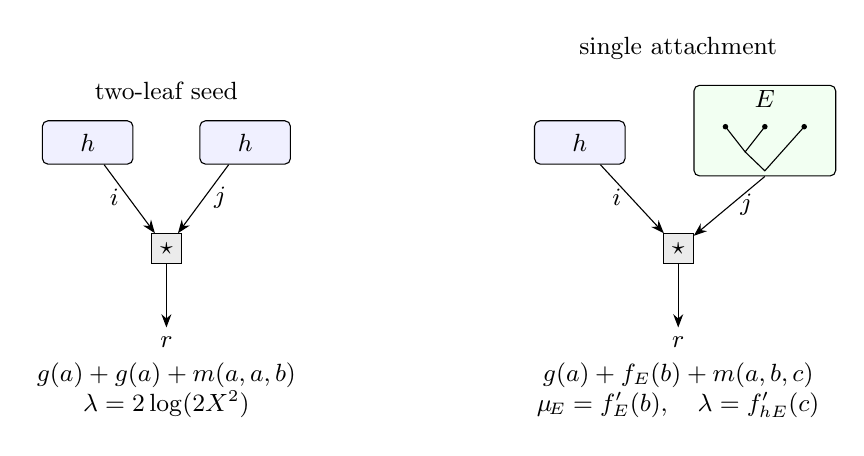
\begin{tikzpicture}[x=1cm,y=1cm,>=Stealth,
  leaf/.style={draw,rounded corners=2pt,fill=blue!6,minimum width=1.15cm,minimum height=.55cm},
  gate/.style={draw,fill=black!8,minimum size=.38cm,inner sep=1pt},
  every node/.style={font=\small}]
\begin{scope}
 \node[leaf] (h1) at (-1,1.35) {$h$};
 \node[leaf] (h2) at (1,1.35) {$h$};
 \node[gate] (g) at (0,0) {$\star$};
 \draw[->] (h1) -- node[left,pos=.48] {$i$} (g);
 \draw[->] (h2) -- node[right,pos=.48] {$j$} (g);
 \draw[->] (g) -- (0,-1) node[below] {$r$};
 \node[align=center] at (0,-1.8) {$g(a)+g(a)+m(a,a,b)$\\$\lambda=2\log(2X^2)$};
 \node at (0,2) {two-leaf seed};
\end{scope}
\begin{scope}[xshift=6.5cm]
 \node[leaf] (h) at (-1.25,1.35) {$h$};
 \node[draw,rounded corners=2pt,fill=green!5,minimum width=1.8cm,minimum height=1.15cm] (E) at (1.1,1.5) {};
 \node at (1.1,1.9) {$E$};
 \fill (.6,1.55) circle (1pt);
 \fill (1.1,1.55) circle (1pt);
 \fill (1.6,1.55) circle (1pt);
 \draw (.6,1.55)--(.85,1.23)--(1.1,1.55);
 \draw (.85,1.23)--(1.1,.99)--(1.6,1.55);
 \node[gate] (g) at (0,0) {$\star$};
 \draw[->] (h) -- node[left,pos=.48] {$i$} (g);
 \draw[->] (E.south) -- node[right,pos=.48] {$j$} (g);
 \draw[->] (g) -- (0,-1) node[below] {$r$};
 \node[align=center] at (0,-1.8) {$g(a)+f_E(b)+m(a,b,c)$\\$\mu_{\!E}=f_E'(b),\quad\lambda=f_{hE}'(c)$};
 \node at (0,2.55) {single attachment};
\end{scope}
\end{tikzpicture}

\caption{A completed construction retains its exact indices at every step; $\star$ is the multiplication in \eqref{cs:product}. In the left seed, $i,j$ are leaf indices and $r$ is the output of their original multiplication. In the right attachment, $j$ is the output of the entire child $E$, not a new leaf. The affine estimates use the same $i/N,j/N,r/N$; the internal slopes cancel at the selected stationary state.}
\label{cs:figure}
\end{figure}

\section{Exact rational verification of the two comparisons}\label{cs:arithmetic}

The two finite supporting-plane arguments use fixed rational points, not numerically located maximizers as hypotheses. This section specifies the data and proves how every transcendental quantity in the comparisons is enclosed. Together with concavity and the exact covers in Sections~\ref{cs:two-leaf} and \ref{cs:attachment}, these are finite proofs of the two inequalities.

The ancillary files in the repository's \texttt{experiments/} directory are
\begin{center}\small
\begin{tabular}{l}
\texttt{conway\_two\_leaf\_block\_alias\_certificate.json}\\
\texttt{conway\_single\_leaf\_attachment\_certificate.json}\\
\texttt{verify\_conway\_two\_leaf\_block\_alias\_certificate.py}\\
\texttt{verify\_conway\_single\_leaf\_attachment\_certificate.py}.
\end{tabular}
\end{center}
The first table records the sixteen slope intervals and three rational points in each. The second records a rooted subdivision tree; a node is either its four quarter-rectangles or one pure point and one alias point. Coordinates are integer multiples of the denominator declared by the table. The verifier checks strict feasibility and the core conditions before taking any derivative. For the first alias profile its core tangent coordinate is strictly between $1/4$ and $1/2$, so the derivative is the stated derivative of $g$.

\subsection{Outward interval arithmetic}
Let $S=10^{40}$. An interval is stored as integers $(l,u)$ representing $[l/S,u/S]$. A rational input is rounded down and up to this grid. Addition and subtraction are exact on the grid. Multiplication uses all four endpoint products with outward integer rounding; division uses all four endpoint quotients after checking that the denominator interval avoids zero. Thus every subsequent interval contains the exact expression, by induction on its arithmetic operations. Repeated multiplication gives nonnegative integer powers.

For the constant $\pi$ use Machin's identity
\[
 \pi=16\arctan(1/5)-4\arctan(1/239).
\]
Truncate each alternating series after 40 terms and enclose its remainder by the absolute next term. The resulting interval also verifies $\pi<22/7$.

For $\sin(\pi t)$, reflect $t>1/2$ to $1-t$ and use the Taylor polynomial through degree 41. On $0\le\pi t\le\pi/2$, its error is at most $(\pi t)^{43}/43!$. Rational interval operations applied to the enclosed $\pi$ give an outward enclosure. Every sine used inside a logarithm is at a strict positive rational argument below one; positivity of its resulting enclosure is checked.

For a positive interval $x$, multiply by a power of two until its lower endpoint is in $[1,2)$. Put $z=(x-1)/(x+1)$ and verify $0\le z<1/2$ throughout the interval. Then
\begin{equation}\label{cs:log-series}
 \log x=2\sum_{j=0}^{79}\frac{z^{2j+1}}{2j+1}+R,
 \qquad 0\le R\le\frac{2z^{161}}{161(1-z^2)}.
\end{equation}
The upper bound follows by replacing every subsequent denominator by 161 and summing the geometric powers. The same formula at $z=1/3$ encloses $\log2$ and restores the extracted power. Monotonicity and outward rounding are used at every step; the small width of the interval is not presumed.

\subsection{The log-sine integral and gradients}
For $0<t<1/2$, integration of the absolutely convergent Euler sine product gives
\begin{equation}\label{cs:J-series}
 J(t)=t\log(2\pi t)-t-
 \sum_{n=1}^{20}\frac{\zeta(2n)t^{2n+1}}{n(2n+1)}-R_t,
 \qquad
 0\le R_t\le\frac{2t^{43}}{21\cdot43(1-t^2)}.
\end{equation}
To justify the expansion directly, write
$\log(\sin\pi u/(\pi u))
=\sum_{k\ge1}\log(1-u^2/k^2)$, expand each negative logarithm and integrate; the nonnegative double series permits termwise integration. For the tail use $\zeta(2n)<2$ and $n(2n+1)\ge21\cdot43$ for $n\ge21$.

The first zeta value is $\zeta(2)=\pi^2/6$. For $2\le n\le20$ integral comparison gives
\[
 \sum_{k=1}^{64}k^{-2n}
 \le\zeta(2n)\le
 \sum_{k=1}^{64}k^{-2n}+
 \frac{64^{1-2n}}{2n-1}.
\]
All these bounds are rational except for the already enclosed $\pi$. Use the exact values of $J$ at $0,1/2,1$, and use $J(1-t)=-J(t)$ above $1/2$.

The gradients needed for the supporting planes contain only positive sines:
\begin{align*}
 m_x&=\log\frac{\sin\pi(x+y)\sin\pi(z-x)}
                     {\sin\pi x\sin\pi(x+y-z)},\\
 m_y&=\log\frac{\sin\pi(x+y)\sin\pi(z-y)}
                     {\sin\pi y\sin\pi(x+y-z)},\\
 m_z&=\log\frac{\sin\pi z\sin\pi(x+y-z)}
                     {\sin\pi(z-x)\sin\pi(z-y)}.
\end{align*}
Together with the displayed derivatives of $g$ and $k$, equations \eqref{cs:log-series} and \eqref{cs:J-series} enclose every term of \eqref{cs:two-certificate} and \eqref{cs:single-certificate}. The lower interval endpoints give precisely the rational margins \eqref{cs:two-margin} and \eqref{cs:single-margin}. Evaluating a tangent at a boundary vertex requires no singular derivative at that vertex: all derivatives are taken at the strict rational tangent point.

The elementary bound \eqref{cs:elementary-margin} can also be checked without special-function evaluation. Its four-term lower sum is
\[
 \frac23-\frac{(2/3)^3}{9}+\frac{(2/3)^5}{25}
 -\frac{(2/3)^7}{49}=\frac{1708762}{2679075}.
\]
For $\log(3/2)$, the first three terms of its $z=1/5$ series and the bound on its remaining positive tail give
\[
 \log(3/2)\le
 2\left(\frac15+\frac{1}{3\cdot5^3}+\frac{1}{5\cdot5^5}\right)
 +\frac{2}{5^7\cdot7(1-1/25)}
 =\frac{177391}{437500}.
\]
Multiplying the first lower bound by $7/11$ and subtracting the second gives the fraction in \eqref{cs:elementary-margin}.

\subsection{Reproduction and the limits of the finite computation}
From the repository root, with Python's standard library alone, run
\begin{verbatim}
python3 papers/conway-source-bounds/check.py \
    --output /tmp/conway-source-check
\end{verbatim}
The wrapper replays the two certificates, verifies their coverage counts
and margins, and checks the elementary rational comparison. It also
calls \texttt{check\_fourier.py}, which compares
\eqref{cs:fourier-exact} with independent monic polynomial division
at \(N=2,\ldots,18\), including unreduced products and multiples of
\(P_N\). The same program checks the rational crossing phases and
angular derivatives, the endpoint-jet repair, and the two-high support
exclusion. Nonzero classes invisible to all spectral values and negative
controls for a nonzero missing winding or deleted normals test the
need to retain the full quotient.

The wrapper records source and data hashes before and after execution.
It rejects optimized Python, runs isolated subprocesses and removes any
old success summary before validation. The output contains both detailed
rational records, the bounded finite-algebra record and a summary.

The computation proves the finite inequalities once the enclosure rules and concavity arguments above have been established. It does not sample levels to prove the Ward identity, the long matrix-product bounds, or the tree induction. Those are all-level written arguments. The physical identification of the finite algebra remains the stated import from \cite{Newton}. Neither the interval certificates nor the bounded Fourier checks replace that identification or prove an analytic estimate by samples.

The theorem can be used in a later filling argument in the following precise way. It supplies a strict bound on the sum of all alias sectors and on the entire physical-color complement of a fixed complete-color neighborhood. A filling analysis must still keep its exact finite functional, control the remaining neighborhood and prove a nonzero selected contribution with the appropriate normalization. These requirements are not conclusions of an absolute source bound.


\begin{thebibliography}{9}
\bibitem{Newton}\emph{Newton coefficients and positive sources for Conway tangles}.
Companion paper, \href{https://sashakolpakov.github.io/murakamis_dream/papers/newton-tangles.pdf}{repository edition}.
\bibitem{Certificates} \emph{Rational supporting-plane data for two-leaf blocks and single-leaf attachments}.
Ancillary data and exact verifiers, \href{https://github.com/sashakolpakov/murakamis_dream/tree/main/experiments}{repository experiments}; the exact filenames and replay are given in Section~\ref{cs:arithmetic}.
\end{thebibliography}
\end{document}
